% !TEX root = ../main.tex
% SECTION 1: ZAHNRÄDER
% Inhalt: Liv Erne, Silvio Seiz — Form: ZSF-Template-Rework
% ============================================================

\StartChapter[ch:zahnradtechnik]{Zahnräder}

\SubsectionBar[sec:zahnrad-grundlagen]{Grundlagen}
\ZSFindex{Leistung}

\begin{formulabox}[Mechanische Leistung]
\[ 1\,\text{W} = 1\;\text{J/s} = 1\;\text{Nm/s} = 60\;\text{Nm/min} \]
\formulasep
\[ \ZSFgearPowerAn = \ZSFgearTorqueOne\cdot\ZSFgearOmegaOne = \ZSFgearTorqueOne \cdot 2\pi\cdot \ZSFgearNOne \]
\[ \ZSFgearPowerAb = \ZSFgearTorqueTwo\cdot\ZSFgearOmegaTwo = \ZSFgearTorqueTwo \cdot 2\pi\cdot \ZSFgearNTwo \]
\formulanote{$\ZSFgearPower{P}$:~Leistung \ $\cdot$ \ $\ZSFgearTorque$:~Moment \ $\cdot$ \ $\ZSFgearSpeed{\omega}$:~Winkelges. \\ $\ZSFgearSpeed{n}$:~Drehzahl \ $\cdot$ \ $1$:~Antrieb, $2$:~Abtrieb}
\end{formulabox}

\begin{runintext}
Bei der Energieumwandlung geht Energie in Form von Wärme verloren. Der \ZSFkeyword{Wirkungsgrad} beschreibt, wie viel der Energie nach der Umwandlung noch in der gewollten Form vorliegt ‒ Reibung im Zahnkontakt führt zu Leistungsverlust:
\end{runintext}

\begin{formulabox}[Wirkungsgrad $\ZSFgearEta$]
\[ \ZSFgearPowerAn \geq \ZSFgearPowerAb \qquad \ZSFgearEta = \frac{\ZSFgearPowerAb}{\ZSFgearPowerAn} \leq 1 \]
\formulanote{Stirnrad: $0{,}96 < \ZSFgearEta < 0{,}99$ \ | \ Kegelrad: $0{,}90 < \ZSFgearEta < 0{,}98$}
\end{formulabox}

\ZSFindex[ubersetzung]{Übersetzung}
\begin{formulabox}[Übersetzung]
\formulanoteabove{Antrieb $=\ZSFgearIndexOne{1}$, Abtrieb $=\ZSFgearIndexTwo{2}$}
\[ \ZSFgearMotion{i_{12}} = \frac{\ZSFgearOmegaOne}{\ZSFgearOmegaTwo} = \frac{\ZSFgearNOne}{\ZSFgearNTwo} = \frac{\ZSFgearDTwo}{\ZSFgearDOne} = \dfrac{\ZSFgearRTwo}{\ZSFgearROne} = \frac{\ZSFgearZTwo}{\ZSFgearZOne} = \frac{\ZSFgearTorqueTwo}{\ZSFgearTorqueOne \cdot \ZSFgearEta} \]
\formulanote{$\ZSFgearMotion{i}$:~Übersetzung $\cdot$ $\ZSFgearSpeed{\omega},\ZSFgearSpeed{n}$:~Winkelgeschwindigkeit/Drehzahl \\ $\ZSFgearD,\ZSFgearR$:~Teilkreisdurchmesser/-radius $\cdot$ $\ZSFgearZ$:~Zähnezahl \\ $\ZSFgearTorque$:~Drehmoment $\cdot$ $\ZSFgearEta$:~Wirkungsgrad (nur bei Moment)}
\formulasep
\[ \ZSFgearMotion{i_{ges}} = \ZSFgearMotion{i_{12}} \cdot \ZSFgearMotion{i_{34}} \cdot \ZSFgearMotion{i_{56}} \cdot \dots \]
\end{formulabox}

\begin{defbox}[Verzahnungsgesetz]
\ZSFindex{Verzahnungsgesetz}
\begin{factlist}
\ZSFFact{Eingriffslinie}{Linie, auf der alle Berührpunkte liegen, wobei der Schnittpunkt mit der Verbindungslinie der beiden Drehzentren der \ZSFkeyword[Walzpunkt@Wälzpunkt]{Wälzpunkt} C ist. Bei der Evolvente ist die Eingriffslinie eine Gerade, womit das Drehmoment und die Drehzahl mit konstanter Übersetzung i übertragen wird. Es gibt auch andere Zahnformen mit gerader Eingriffslinie.}
\ZSFFact{Evolvente}{Durch die Evolventenform geht die Normale im Berührungspunkt immer durch den Wälzpunkt C, siehe Eingriffslinie.}
\ZSFFact{Modul}{Der Modul ($\ZSFgearM$, Zahngrösse) ist die Segmentgrösse, also wieviel Platz ein Zahn benötigt. Nur Zahnräder mit gleichem Modul $\ZSFgearMOne = \ZSFgearMTwo$ können kombiniert werden.}
\ZSFFact{Wälzen}{Kombination von Rollen und Gleiten im Zahnradeingriff führt zu Reibung an der Zahnflanken.}
\end{factlist}
\end{defbox}
\ZSFindex{Eingriffslinie}
\ZSFindex{Evolvente}
\ZSFindex{Modul}
\ZSFindex[walzen]{Wälzen}

\begin{splitbox}[0.53]
\centering
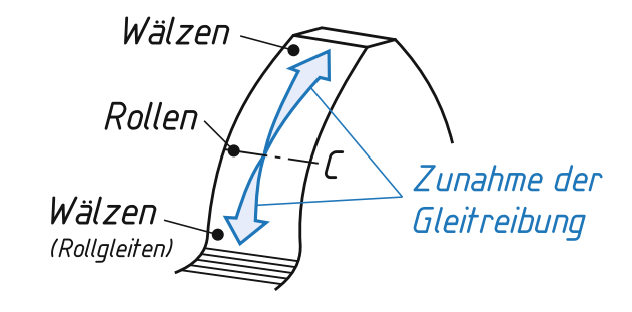
\includegraphics[width=\linewidth,keepaspectratio]{graphics/gear_rolling_process.png}
\tcblower
\textbf{\ZSFkeyword*{Spezifisches Gleiten}} $\ZSFgearSlip$:~\ZSFgapXS
{\centering $\displaystyle |\ZSFgearSlip| = \frac{\ZSFgearVSliding}{\ZSFgearVRolling} \leq 2$\par}
\ZSFgapS
Am Wälzpunkt tritt\\
reines Rollen auf, $\ZSFgearSlip = 0$.
\ZSFgapS
$|\ZSFgearSlip|$ ist maximal beim\\
Eingriffsbeginn und -Ende.
\end{splitbox}
\ZSFindex{Gleiten, spezifisches}

\SubsectionBar[sec:stirnzahnradtechnik]{Stirnzahnräder}
\ZSFindex{Stirnzahnrad}

\ZSFfig[1.0]{graphics/stirnrad_kennwerte_zahngeometrie.png}{Kennwerte Stirnrad}{}

\SubsubsectionBarOnNewColumn*{Normzahnräder}
\begin{figbox}[]
  \noindent
  \begin{minipage}[c]{0.45\linewidth}%
    \centering
    \begin{tikzpicture}[x=0.75pt, y=0.75pt, >=latex, font=\sffamily\fontsize{5.5}{6.5}\selectfont]
      % 1. Fill gear bodies
      \fill[GearObjOneColor!8] (20, 14) rectangle (60, 30);
      \fill[GearObjTwoColor!8] (50, 14) rectangle (100, 30);

      % 2. Draw solid boundaries of Gear 1 (left/top/bottom up to contact)
      \draw[thick, GearObjOneColor] (20, 14) -- (55, 14);
      \draw[thick, GearObjOneColor] (20, 30) -- (55, 30);
      \draw[thick, GearObjOneColor] (20, 14) -- (20, 30);

      % 3. Draw dashed boundaries of Gear 1 (inside Gear 2)
      \draw[thick, GearObjOneColor, dashed] (55, 14) -- (60, 14);
      \draw[thick, GearObjOneColor, dashed] (55, 30) -- (60, 30);
      \draw[thick, GearObjOneColor, dashed] (60, 14) -- (60, 30);

      % 4. Draw solid boundaries of Gear 2 (right/top/bottom from contact)
      \draw[thick, GearObjTwoColor] (55, 14) -- (100, 14);
      \draw[thick, GearObjTwoColor] (55, 30) -- (100, 30);
      \draw[thick, GearObjTwoColor] (100, 14) -- (100, 30);

      % 5. Draw dashed boundaries of Gear 2 (inside Gear 1)
      \draw[thick, GearObjTwoColor, dashed] (50, 14) -- (55, 14);
      \draw[thick, GearObjTwoColor, dashed] (50, 30) -- (55, 30);
      \draw[thick, GearObjTwoColor, dashed] (50, 14) -- (50, 30);

      % 6. Draw vertical dashed-dotted lines (pitch lines and axes)
      \draw[dashdotted, black!60, semithick] (25, 9) -- (25, 35);
      \draw[dashdotted, black!60, semithick] (40, 5) -- (40, 38);
      \draw[dashdotted, black!60, semithick] (55, 5) -- (55, 38);
      \draw[dashdotted, black!60, semithick] (75, 5) -- (75, 38);
      \draw[dashdotted, black!60, semithick] (95, 9) -- (95, 35);

      % 7. Draw solid vertical extension lines (Hilfslinien) for all dimensions
      \draw[thick, GearVarHeightHeadColor!70] (20, 14) -- (20, 7);
      \draw[thick, GearVarHeightHeadColor!70] (25, 14) -- (25, 7);
      \draw[black!40] (40, 14) -- (40, 1);
      \draw[black!40] (55, 14) -- (55, 7);
      \draw[black!40] (75, 14) -- (75, 1);
      \draw[thick, GearVarHeightHeadColor!70] (95, 14) -- (95, 7);
      \draw[thick, GearVarHeightHeadColor!70] (100, 14) -- (100, 7);

      % 8. Dimension lines with arrowheads / ticks
      \draw[<->, >=stealth, black!60] (25, 8) -- (55, 8);
      \draw[<->, >=stealth, black!60] (55, 8) -- (95, 8);
      \draw[<->, >=stealth, black!60] (40, 2) -- (75, 2);
      
      \draw[thick, GearVarHeightHeadColor] (20, 8) -- (25, 8);
      \draw[thick, GearVarHeightHeadColor] (20, 7.2) -- (20, 8.8);
      \draw[thick, GearVarHeightHeadColor] (25, 7.2) -- (25, 8.8);
      
      \draw[thick, GearVarHeightHeadColor] (95, 8) -- (100, 8);
      \draw[thick, GearVarHeightHeadColor] (95, 7.2) -- (95, 8.8);
      \draw[thick, GearVarHeightHeadColor] (100, 7.2) -- (100, 8.8);

      % 9. Draw labels inside the gear bodies
      \node[GearObjOneColor, font=\bfseries] at (40, 22) {1};
      \node[GearObjTwoColor, font=\bfseries] at (75, 22) {2};

      % 10. Draw dimension labels LAST with background masking fill
      \node[fill=\FigboxBackColor, inner sep=1.5pt] at (40, 8) {$\ZSFgearDOne$};
      \node[fill=\FigboxBackColor, inner sep=1.5pt] at (75, 8) {$\ZSFgearDTwo$};
      \node[fill=\FigboxBackColor, inner sep=1.5pt] at (57.5, 2) {$\ZSFgearAd$};

      \node[scale=0.85] at (22.5, 3.2) {$\ZSFgearHeightHead{h_{a\ZSFgearIndexOne{1}}} = \ZSFgearModule{m}$};
      \node[scale=0.85] at (97.5, 3.2) {$\ZSFgearHeightHead{h_{a\ZSFgearIndexTwo{2}}} = \ZSFgearModule{m}$};
    \end{tikzpicture}
  \end{minipage}%
  \hfill
  \begin{minipage}[c]{\dimexpr0.96\linewidth-0.45\linewidth\relax}%
    \raggedright
    \ZSFReadableOn
    \ZSFkeyword{Eingriffswinkel}:\\
    $\ZSFgearAlpha = 20^\circ$
    \ZSFgapXS

    {\centering $\displaystyle \ZSFgearAd = \frac{\ZSFgearDOne + \ZSFgearDTwo}{2} = \frac{\ZSFgearM\cdot(\ZSFgearZOne + \ZSFgearZTwo)}{2}$\par}
    \ZSFgapXS

    {\centering $\displaystyle \ZSFgearU = \ZSFgearP \cdot \ZSFgearZ = \ZSFgearD\cdot\pi$\par}
  \end{minipage}%
  \par
\end{figbox}

\phantomsection\label{formula:gear-normal-geometry}
\begin{formulabox}[Geometrie]
\[ \ZSFgearHa = \ZSFgearM \qquad \ZSFgearHf = 1,1 \dots 1,3 \cdot \ZSFgearM \qquad \ZSFgearH = \ZSFgearHa + \ZSFgearHf \]
\[ \ZSFgearDf = \ZSFgearD - 2\cdot \ZSFgearHf \qquad \ZSFgearD = \ZSFgearZ \cdot \ZSFgearM = \ZSFgearZ \cdot \dfrac{\ZSFgearP}{\pi} \]
\[ \ZSFgearDa = \ZSFgearD + 2\cdot \ZSFgearHa = \ZSFgearD + 2\cdot \ZSFgearM \qquad \ZSFgearDb =\ZSFgearD\cdot\cos\ZSFgearAlpha \]
\formulanote{%
$\ZSFgearAd$:~Null-Achsabstand $\cdot$ $\ZSFgearU$:~Umfang $\cdot$ $\ZSFgearAlpha$:~Eingriffswinkel ($20^\circ$) \\
$\ZSFgearHa$:~Kopfhöhe $\cdot$ $\ZSFgearHf$:~Fusshöhe $\cdot$ $\ZSFgearH$:~Zahnhöhe $\cdot$ $\ZSFgearM$:~Modul $\cdot$ $\ZSFgearP$:~Teilung $\cdot$ $\ZSFgearZ$:~Zähnezahl \\
$\ZSFgearD$:~Teilkreis- $\cdot$ $\ZSFgearDf$:~Fusskreis- $\cdot$ $\ZSFgearDa$:~Kopfkreis- $\cdot$ $\ZSFgearDb$:~Grundkreisdurchmesser%
}
\end{formulabox}

\ZSFindex[grenzzahnezahl]{Grenzzähnezahl}
\begin{formulabox}[Grenzzähnezahl]
\formulanoteabove{Theoretische $\ZSFgearZg$ und praktische $\ZSFgearZgPrime$ Grenzzähnezahl:}
\[ \ZSFgearZg = 17 \text{ und } \ZSFgearZgPrime = 14 \text{ für } \ZSFgearAlpha = 20° \qquad \ZSFgearZg = \frac{2}{sin^2\ZSFgearAlpha} \]
\formulanote{Die maximale Übersetzung wird mit dem kleinsten zulässigen Zahnrad (14 Zähne) und dem grössten möglichen Zahnrad erreicht.}
\end{formulabox}

\SubsubsectionBar{Profilüberdeckung}
\ZSFindex[profiluberdeckung]{Profilüberdeckung}

\begin{runintext}
Beschreibt wieviele Zähne gleichzeitig im Eingriff sind, mit Eingriffsstrecke $\ZSFgearGalpha$ und Eingriffsteilung $\ZSFgearPe$.
\end{runintext}

\begin{formulabox}
\formulasources{$\ZSFgearDa$, $\ZSFgearDb$:~Normrad \ZSFsource{aus}{formula:gear-normal-geometry}, profilversch. \ZSFsource{aus}{formula:gear-profile-shift}}
\formulanoteabove{%
Bei Schrägverzahnung: Überdeckungsformeln \ZSFref{sec:schraegverzahnung}.}
\[ \ZSFgearEpsAlpha = \frac{\ZSFgearGalpha}{\ZSFgearPe} = \frac{\frac{1}{2}\cdot(\sqrt{\ZSFgearDaOne^2-\ZSFgearDbOne^2}+\sqrt{\ZSFgearDaTwo^2-\ZSFgearDbTwo^2}) - \ZSFgearAd\cdot \sin\ZSFgearAlpha}{\pi\cdot \ZSFgearM\cdot\cos\ZSFgearAlpha} \]
\formulanote{$\ZSFgearEpsAlpha$:~Profilüberdeckung $\cdot$ $\ZSFgearGalpha$:~Eingriffsstrecke $\cdot$ $\ZSFgearPe$:~Eingriffsteilung \\ $\ZSFgearAd$:~Null-Achsabstand $\cdot$ $\ZSFgearAlpha$:~Eingriffswinkel ($20^\circ$) $\cdot$ $\ZSFgearM$:~Modul}
\end{formulabox}
\begin{statementbox}[Eigenschaften und Richtwerte]
\ZSFReadableOn
Bei grossem $\ZSFgearEpsAlpha$:~\begin{factlist}
\item vibrationsärmer und leiser
\item höhere Lebensdauer und Tragfähigkeit
\end{factlist}
\ZSFgapS
Richtwerte $\ZSFgearEpsAlpha$:~\begin{factlist}
\item \textbf{Nicht zulässig} (kein Zahnkontakt): $\ZSFgearEpsAlphaBrace < 1.0$
\item \textbf{Industriestandard}:~$1.3 \leq \ZSFgearEpsAlpha \leq 1.6$
\item \textbf{Sehr ruhiger Lauf}:~$\ZSFgearEpsAlphaBrace \geq 1.6$
\end{factlist}
\end{statementbox}

\SubsubsectionBar{Profilverschiebung}
\ZSFindex{Profilverschiebung}

\begin{runintext}
Verhältnis von aufsteigender zu absteigender Flanke (Grundkreis $\ZSFgearDb$ bis Kopfkreis $\ZSFgearDa$). Dabei ändern sich der Achsenabstand $\ZSFgearA$ und Eingriffswinkel $\ZSFgearAlpha$.
\end{runintext}

\begin{factlist}
\ZSFFact{Kleine Flanke/ viel Unterschnitt}{Geschwächter Zahnfuss durch Biegemoment}
\ZSFFact{Grosse Flanke/ wenig Unterschnitt}{Zahn wird spitz, also kein Platz für gegenüberliegenden Zahn}
\end{factlist}

\phantomsection\label{formula:gear-profile-shift}
\begin{formulabox}[Profilverschiebungsfaktor $\ZSFgearX$]
\[
\begin{array}{ll}
  \ZSFgearVplus\text{-Rad: } \ZSFgearX > 0 \ (s\uparrow, \text{Unterschnitt}\downarrow) & \quad \big| \quad \text{Null-Rad: } \ZSFgearX = 0 \\
  \ZSFgearVminus\text{-Rad: } \ZSFgearX < 0 \ (s\downarrow, \text{Unterschnitt}\uparrow) &
\end{array}
\]
\formulasep
\[ \ZSFgearX = \frac{\ZSFgearV}{\ZSFgearM} \qquad \ZSFgearDa = \ZSFgearD + 2\ZSFgearM + 2\ZSFgearV = \ZSFgearD + 2\cdot \ZSFgearM\cdot (1+\ZSFgearX) \]
\formulanote{$\ZSFgearX$:~Profilverschiebungsfaktor $\cdot$ $\ZSFgearV$:~Verschiebung (beidseitig $\Rightarrow 2\cdot \ZSFgearV$) \\ $\ZSFgearM$:~Modul $\cdot$ $\ZSFgearD, \ZSFgearDa$:~Teilkreis-/Kopfkreisdurchmesser}
\end{formulabox}

\SubsubsectionBar[sec:geradverzahnung]{Geradverzahnung Kräfte}
\ZSFindex{Geradverzahnung}

\begin{splitbox}[0.57]
\centering
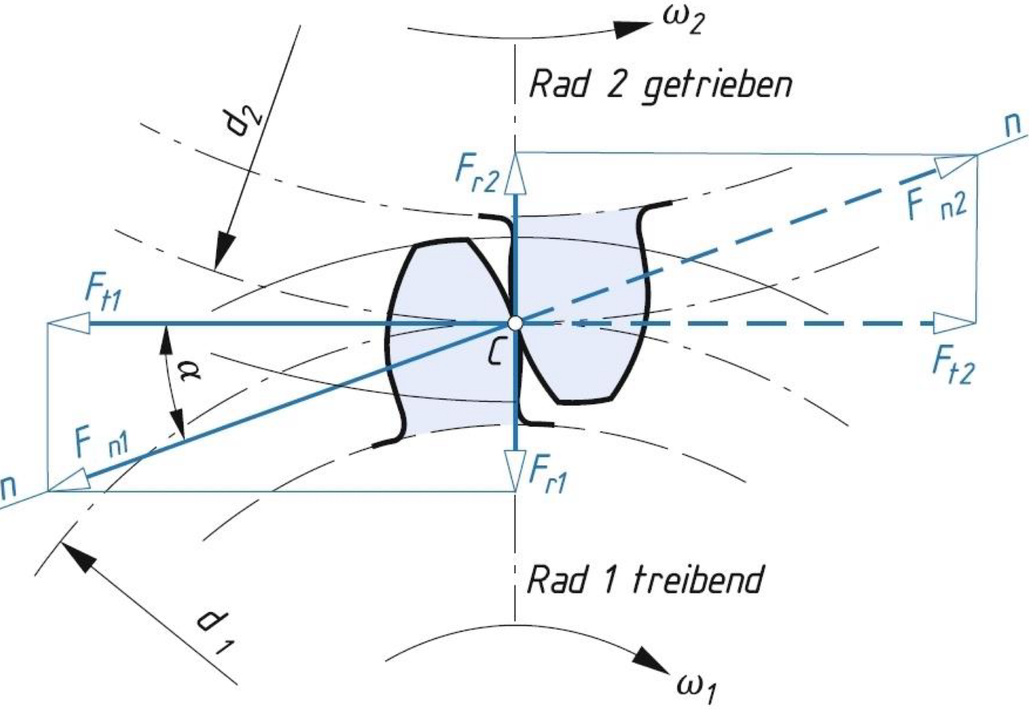
\includegraphics[width=\linewidth,keepaspectratio]{graphics/spur_gear_contact_forces_line_of_action.png}
\tcblower
Getriebenes Rad:

$\ZSFgearFtTwo = \ZSFgearFtOne$ \quad $\ZSFgearFrTwo = \ZSFgearFrOne$
\ZSFgapS

Treibendes Rad:

$\ZSFgearFtOne = \frac{\ZSFgearTorqueOne}{\ZSFgearROne} = \frac{2\cdot \ZSFgearTorqueOne}{\ZSFgearDOne}$

$\ZSFgearFrOne = \ZSFgearFtOne \cdot \tan\ZSFgearAlpha$

$\ZSFgearFn = \dfrac{\ZSFgearFt}{\cos\ZSFgearAlpha}$
\ZSFgapXS

\formulanote{%
$\ZSFgearFt$:~Tangentialkraft \\
$\ZSFgearFr$:~Radialkraft \\
$\ZSFgearFn$:~Normalkraft \\
$\ZSFgearTorque$:~Drehmoment \\
$\ZSFgearR,\ZSFgearD$:~Teilkreis- $r,d$ \\
$\ZSFgearAlpha$:~Eingriffswinkel ($20^\circ$) \\
bei Welle siehe \ZSFref{sec:biegung}%
}
\end{splitbox}

\begin{statementbox}[Kraftrichtung]
Antrieb: $\ZSFgearFrOne$ nach innen zum Antrieb, $\ZSFgearFtOne$ entgegen der Drehrichtung, $\ZSFgearFrTwo$ und $\ZSFgearFtTwo$ entgegen der $\ZSFgearFOne$ Kräfte
\end{statementbox}

\SubsubsectionBarOnNewColumn{V-Getriebe}
\ZSFindex{V-Getriebe}

\begin{runintext}
$\sum \ZSFgearX \neq 0$ und $\ZSFgearAlpha$ wird zum \ZSFkeyword{Betriebswinkel} $\ZSFgearAlphaW$.
\end{runintext}

\begin{figbox}[V-Getriebe]
  \noindent
  \begin{minipage}[c]{0.68\linewidth}
    \raggedright
    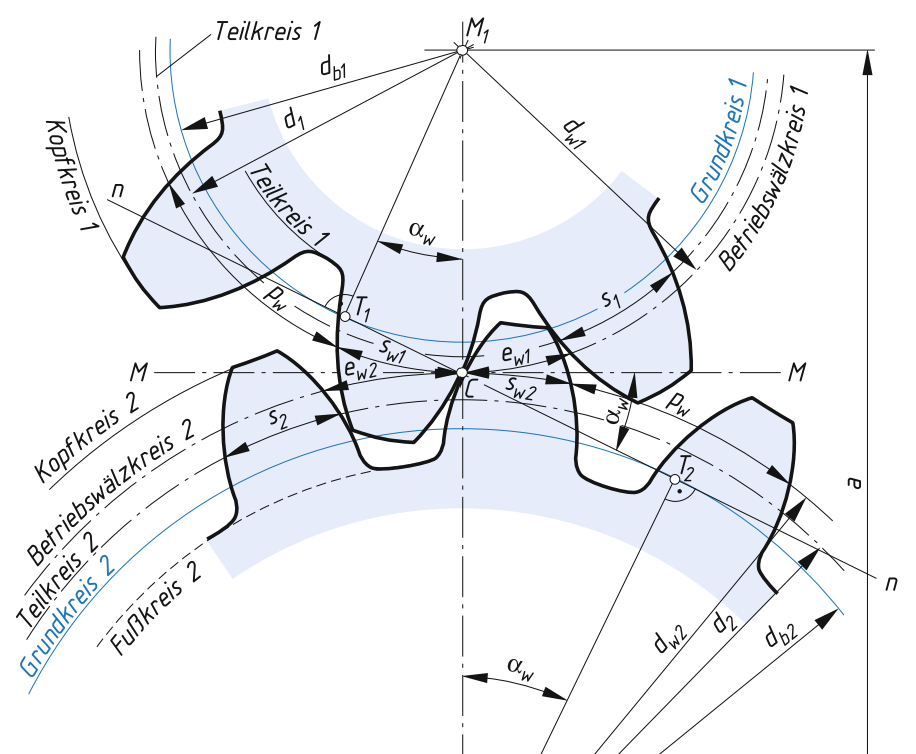
\includegraphics[width=\linewidth,keepaspectratio]{graphics/v_getriebe_kennwerte.png}
  \end{minipage}%
  \begin{minipage}[c]{0.31\linewidth}
    \centering
    $\ZSFgearSwOne = \ZSFgearEwTwo$, $\ZSFgearSwTwo = \ZSFgearEwOne$ \\[2pt]
    $\ZSFgearA = \ZSFgearAd \cdot\frac{\cos\ZSFgearAlpha}{\cos\ZSFgearAlphaW} = \ZSFgearAd + \Delta{\ZSFgearA}$ \\[3pt]
    {\ZSFfontNote $\ZSFgearSw/\ZSFgearEw$:~Wälzzahndicke/-lücke \\ $\ZSFgearA,\ZSFgearAd$:~Betriebs-/Null-Achsabstand \\ $\ZSFgearAlphaW$:~Betriebseingriffswinkel \\ $\Delta\ZSFgearA$:~Achsabstandsänderung\par}
  \end{minipage}
\end{figbox}

\begin{defbox}[Bestimmung Betriebswinkel $\ZSFgearAlphaW$]
\begin{enumerate}[leftmargin=1.1em,itemsep=0.5pt,topsep=1.5pt,parsep=0pt]
  \item $\text{inv}\,\ZSFgearAlpha = \tan\ZSFgearAlpha - \ZSFgearAlpha\cdot(\frac{\pi}{180°})$ \hfill (\small$\text{inv}\,(20°) = 0.0149$)
  \item $\text{inv}\,\ZSFgearAlphaW = 2\,\frac{\ZSFgearXOne+\ZSFgearXTwo}{\ZSFgearZOne+\ZSFgearZTwo}\,\cdot \tan\ZSFgearAlpha + \text{inv}\,\ZSFgearAlpha$
  \item $\ZSFgearAlphaW \approx (\sqrt[3]{3 \cdot \text{inv}\,\ZSFgearAlphaW} - \frac{2}{5}\text{inv}\,\ZSFgearAlphaW)\cdot (\frac{180°}{\pi})$
\end{enumerate}
\ZSFgapS
\textbf{Umgestellt:}
{\centering
$\sum \ZSFgearX = \dfrac{(\text{inv}\,\ZSFgearAlphaW - \text{inv}\,\ZSFgearAlpha)\cdot(\ZSFgearZOne+\ZSFgearZTwo)}{2 \cdot \tan\ZSFgearAlpha}$ \\[4pt]
$\ZSFgearAlphaW = \cos^{-1}\left(\frac{\ZSFgearAd}{\ZSFgearA}\cdot \cos\ZSFgearAlpha\right)$ \par}
\formulanote{$\ZSFgearAlpha$:~Eingriffswinkel ($20^\circ$) $\cdot$ $\ZSFgearAlphaW$:~Betriebseingriffswinkel \\ $\sum \ZSFgearX$:~Summe Profilverschiebung $\cdot$ $\ZSFgearZ$:~Zähnezahl}
\end{defbox}

\SubsubsectionBar{V-Null-Getriebe}
\ZSFindex{V-Null-Getriebe}

\begin{formulabox}
\[ \ZSFgearAd = \ZSFgearA = \frac{\ZSFgearDOne + \ZSFgearDTwo}{2} = \ZSFgearROne + \ZSFgearRTwo \text{ und } \sum \ZSFgearX = 0 \]
\formulanote{$\ZSFgearAd, \ZSFgearA$:~Null-/Betriebsachsabstand $\cdot$ $\ZSFgearD, \ZSFgearR$:~Teilkreisdurchmesser/-radius \\ $\ZSFgearX$:~Profilverschiebung $\cdot$ $\ZSFgearS$:~Zahndicke}
\formulanote{$\sum \ZSFgearX=0\Rightarrow \ZSFgearA=\ZSFgearAd,\ZSFgearAlphaW=\ZSFgearAlpha$; $\ZSFgearXOne>0\Rightarrow \ZSFgearSOne\uparrow$, Unterschnitt $\downarrow$; $\ZSFgearXTwo=-\ZSFgearXOne\Rightarrow \ZSFgearSTwo\downarrow$}
\end{formulabox}

\ZSFfig[1.0]{graphics/v_null_gears_characteristics.png}{V-Null-Räder}{} % chktex 25

\SubsubsectionBar[sec:schraegverzahnung]{Schrägverzahnung}
\ZSFindex[schragverzahnung]{Schrägverzahnung}

\begin{runintext}
Durch den \ZSFkeyword{Schrägungswinkel} $\ZSFgearBeta$ sind immer mehrere Zähne durch kontinuierliches Anlegen und Ablösen im Eingriff, anders als bei der Geradverzahnung. Dies ermöglicht einen kontinuierlichen Krafteinfluss und somit höhere Laufruhe und Belastbarkeit.
\end{runintext}

\begin{figbox}[Schrägverzahnung]
\centering
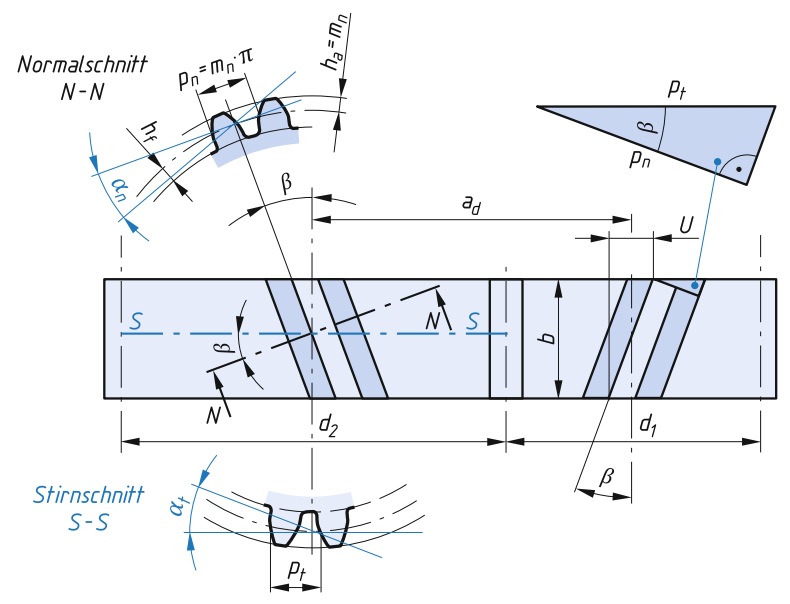
\includegraphics[width=0.73\linewidth,keepaspectratio]{graphics/helical_gear_characteristics.png}%
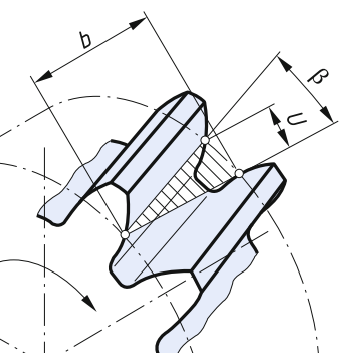
\includegraphics[width=0.25\linewidth,keepaspectratio]{graphics/helical_gear_tooth_contact_detail.png}
\end{figbox}

\phantomsection\label{formula:gear-helical-geometry}
\begin{formulabox}[Geometrie]
\[ \ZSFgearAlphaT = \tan^{-1}(\frac{\tan\ZSFgearAlphaN}{\cos{\ZSFgearBeta}}) \qquad \cos\ZSFgearBeta = \frac{\tan\ZSFgearAlphaN}{\tan\ZSFgearAlphaT} \]
\[ \ZSFgearHa = \ZSFgearMn \qquad \ZSFgearMt = \frac{\ZSFgearMn}{\cos\ZSFgearBeta} = \frac{\ZSFgearD}{\ZSFgearZ} \]
\[ \ZSFgearD = \ZSFgearMt \cdot \ZSFgearZ = \frac{\ZSFgearZ \cdot \ZSFgearMn}{cos\ZSFgearBeta} \]
\[ \ZSFgearDb = \ZSFgearD \cdot\cos\ZSFgearAlphaT = \frac{\ZSFgearZ\cdot \ZSFgearMn \cdot \cos\ZSFgearAlphaT}{\cos\ZSFgearBeta} \]
\[ \ZSFgearDa = \ZSFgearD + 2\cdot \ZSFgearHa = \ZSFgearD + 2\cdot \ZSFgearMn = \ZSFgearMn\cdot \left(2+\frac{\ZSFgearZ}{\cos\ZSFgearBeta}\right) \]
\[ \ZSFgearDf = \ZSFgearD - 2\cdot \ZSFgearHf = \ZSFgearD - 2.5 \cdot \ZSFgearMn \qquad \ZSFgearHf = 1{,}25\cdot \ZSFgearMn \]
\[ \ZSFgearAd = \frac{\ZSFgearDOne + \ZSFgearDTwo}{2}= \ZSFgearMt\cdot\frac{\ZSFgearZOne+\ZSFgearZTwo}{2} = \frac{\ZSFgearMn}{\cos\ZSFgearBeta}\cdot\frac{\ZSFgearZOne + \ZSFgearZTwo}{2} \]
\formulanote{$\ZSFgearMn$:~Normal- / $\ZSFgearMt$:~Stirnmodul \ $\cdot$ \ $\ZSFgearBeta$:~Schrägungswinkel \ $\cdot$ \ $\ZSFgearAlphaN$:~Normal- / $\ZSFgearAlphaT$:~Stirneingriffswinkel \ $\cdot$ \ $\ZSFgearAlphaWT$:~Betriebseingriffswinkel im Stirnschnitt}
\end{formulabox}

\begin{formulabox}[Überdeckungen]
\formulasources{Geometriegrössen: \ZSFsource{aus}{formula:gear-helical-geometry}}
\formulanoteabove{Null-Schrägverzahnung:}
\[ \ZSFgearEpsAlpha = \frac{\ZSFgearGalpha}{\ZSFgearPe} = \frac{\frac{1}{2}\cdot(\sqrt{\ZSFgearDaOne^2-\ZSFgearDbOne^2}+\sqrt{\ZSFgearDaTwo^2-\ZSFgearDbTwo^2}) - \ZSFgearAd\cdot \sin\ZSFgearAlphaT}{\pi\cdot \ZSFgearMt\cdot\cos\ZSFgearAlphaT} \]
\formulanoteabove{V-Schrägverzahnung:}
\[ \ZSFgearEpsAlpha = \frac{\ZSFgearGalpha}{\ZSFgearPe} = \frac{\frac{1}{2}\cdot(\sqrt{\ZSFgearDaOne^2-\ZSFgearDbOne^2}+\sqrt{\ZSFgearDaTwo^2-\ZSFgearDbTwo^2}) - \ZSFgearA\cdot \sin\ZSFgearAlphaWT}{\pi\cdot \ZSFgearMt\cdot\cos\ZSFgearAlphaT} \]
\end{formulabox}

% Spalten-Packung (6-Seiten-Ziel): eine Überdeckungs-Box in zwei geteilt,
% damit die Teile an Spaltenenden umbruchfähig sind. Inhalt unverändert.
\begin{formulabox}[Sprung- und Gesamtüberdeckung]
\[ \ZSFgearEpsBeta = \frac{\ZSFgearUJump}{\ZSFgearPt} = \frac{\ZSFgearB \cdot \tan\ZSFgearBeta}{\ZSFgearPt} = \frac{\ZSFgearB \cdot \tan\ZSFgearBeta}{\pi \cdot \ZSFgearMt} = \frac{\ZSFgearB \cdot \sin\ZSFgearBeta}{\pi \cdot \ZSFgearMn} \]
\[ \ZSFgearEpsGamma = \ZSFgearEpsAlpha + \ZSFgearEpsBeta \]
\end{formulabox}

% Spalten-Packung (6-Seiten-Ziel): Box geteilt. Inhalt unverändert.
\begin{formulabox}
\[ \ZSFgearA = \ZSFgearAd \cdot\frac{cos\ZSFgearAlpha}{cos\ZSFgearAlphaW} = \ZSFgearAd \cdot\frac{cos\ZSFgearAlphaT}{cos\ZSFgearAlphaWT} \]
\[ \ZSFgearC = 0{,}25\cdot \ZSFgearMn \qquad \ZSFgearUJump = \ZSFgearB \cdot \tan\ZSFgearBeta \qquad \ZSFgearZgtPrime = 14 \cdot \cos^3\!\ZSFgearBeta \]
\formulanote{$\ZSFgearC$:~Kopfspiel \ $\cdot$ \ $\ZSFgearUJump$:~Sprung \ $\cdot$ \ $\ZSFgearEpsAll$:~Profil-/Sprung-/Gesamtüberdeckung \ $\cdot$ \ $\ZSFgearZgtPrime$:~Grenzzähnezahl \ $\cdot$ \ $\ZSFgearB$:~Zahnbreite \ $\cdot$ \ $\ZSFgearPt$:~Stirnteilung}
\end{formulabox}
\ZSFindex[sprunguberdeckung]{Sprungüberdeckung}

\begin{figbox}[Kräfte an der Schrägverzahnung]
\centering
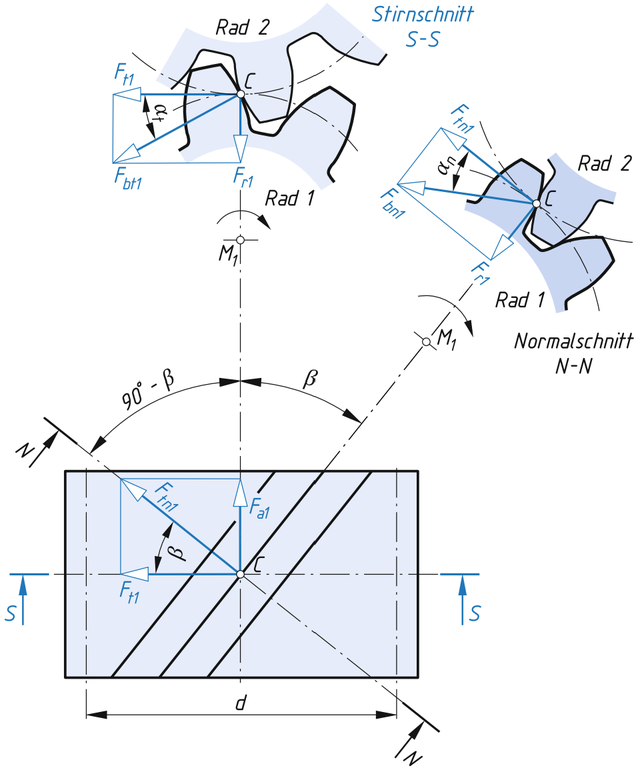
\includegraphics[width=0.62\linewidth,keepaspectratio]{graphics/helical_gear_forces.png}%
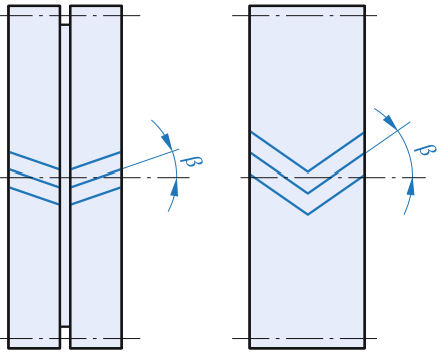
\includegraphics[width=0.38\linewidth,keepaspectratio]{graphics/helical_herringbone_gear_comparison.png}
\end{figbox}

\begin{formulabox}[Kräfte]
\[ \ZSFgearFtOne = \ZSFgearFtTwo = \frac{2\cdot \ZSFgearTorqueOne}{\ZSFgearDOne} \qquad \ZSFgearFaOne = \ZSFgearFaTwo = \ZSFgearFtOne \cdot \tan\ZSFgearBeta \]
\[ \ZSFgearFrOne = \ZSFgearFrTwo = \ZSFgearFtnOne \cdot \tan \ZSFgearAlphaN \ \text{ mit } \ \ZSFgearFtnOne = \frac{\ZSFgearFtOne}{\cos\ZSFgearBeta} \]
\formulanote{bei Welle siehe \ZSFref{sec:biegung} Biegung}
\end{formulabox}

\begin{runintext}
Axialkraft lässt sich durch Doppelschräg- oder \ZSFkeyword{Pfeilverzahnung} aufheben (siehe Bild oben).
\end{runintext}

\SubsectionBar[sec:kegelzahnradtechnik]{Kegelzahnräder}
\ZSFindex{Kegelzahnrad}
\ZSFindexsee{Kegelrad}{Kegelzahnrad}

\begin{runintext}
Umlenkung einer Drehbewegung um einen Winkel $\ZSFgearSigmaAngle$. Falls Zahnrad 1 und 2 baugleich sind: $\ZSFgearDeltaOne = \ZSFgearDeltaTwo$
\end{runintext}

\begin{formulabox}[Übersetzung und Kegelwinkel]
\[ \ZSFgearMotion{i} = \frac{\ZSFgearNOne}{\ZSFgearNTwo} = \frac{\ZSFgearDmTwo}{\ZSFgearDmOne} = \frac{\ZSFgearDeTwo}{\ZSFgearDeOne} = \frac{\ZSFgearZTwo}{\ZSFgearZOne} = \frac{\sin\ZSFgearDeltaTwo}{\sin\ZSFgearDeltaOne} = \frac{\ZSFgearTorqueTwo}{\ZSFgearTorqueOne} \]
\[ \ZSFgearSigmaAngle = \ZSFgearDeltaOne + \ZSFgearDeltaTwo \]
\end{formulabox}

\begin{formulabox}[Kegelwinkel $\ZSFgearDeltaOne$ bestimmen]
\[ \text{Für } \ZSFgearSigmaAngle \leq 90°: \ \tan\ZSFgearDeltaOne = \frac{\sin\ZSFgearSigmaAngle}{\ZSFgearMotion{i}+\cos\ZSFgearSigmaAngle} \]
\[ \text{Für } \ZSFgearSigmaAngle > 90°: \ \tan\ZSFgearDeltaOne = \frac{\sin\ (180°- \ZSFgearSigmaAngle)}{\ZSFgearMotion{i}-\cos\ (180° - \ZSFgearSigmaAngle)} \]
\end{formulabox}

\ZSFfig[0.75]{graphics/kegelradgetriebe_kennwerte_kegelradpaar.png}{Kennwerte Kegelradgetriebe}{}

\ZSFfig[0.84]{graphics/bevel_gear_pair_forces.png}{Kräfte am Kegelradpaar}{}

\begin{formulabox}[Kräfte]
\[ \ZSFgearFmtOne = \frac{2 \cdot \ZSFgearTorqueOne}{\ZSFgearDmOne} \qquad \ZSFgearFrOne = \ZSFgearFmtOne \cdot \tan\ZSFgearAlpha \cdot\cos\ZSFgearDeltaOne \]
\[ \ZSFgearFaOne = \ZSFgearFmtOne \cdot \tan\ZSFgearAlpha \cdot \sin\ZSFgearDeltaOne \]
\[ \ZSFgearFmtTwo = \ZSFgearFmtOne \qquad \ZSFgearFrTwo = \ZSFgearFmtOne\cdot \tan \ZSFgearAlpha \cdot\cos\ZSFgearDeltaTwo \]
\[ \ZSFgearFaTwo = \ZSFgearFmtOne \cdot \tan\ZSFgearAlpha \cdot \sin\ZSFgearDeltaTwo \]
\end{formulabox}

\SubsectionBar[sec:getriebe]{Getriebe}
\ZSFindex{Getriebe}

\begin{runintext}
Spannung $\Leftrightarrow$ Geometrie $\Leftrightarrow$ Kräfte
\end{runintext}

\begin{formulabox}
\[ \ZSFgearMotion{i_{ges}} = \frac{\ZSFgearNAn}{\ZSFgearNAb} \qquad \ZSFgearPsid = \frac{\ZSFgearB}{\ZSFgearDOne} = \frac{\ZSFgearB}{\ZSFgearM \cdot \ZSFgearZOne} \]
\end{formulabox}

\begin{propertylist}[Kausalität]
\ZSFFact{Welle}{Minimaler Zahnrad-Innendurchmesser $\ZSFgearDsh$}
\ZSFFact{Übersetzung}{Zähnezahlverhältnis}
\ZSFFact{Zähnezahl}{Laufruhe und Untergrenze für Modul}
\ZSFFact{Breite}{Tragfähigkeit}
\ZSFFact{Schrägung}{Laufruhe, Momente und Axialkräfte}
\ZSFFact{Modul}{Verknüpfung Zahnradgeometrie mit Materialkennwerten}
\end{propertylist}

\begin{statementbox}[Modulwahl]
\ZSFindex{Modulwahl}
\begin{factlist}
\item Keine plastische Verformungen
\item Kein statischer Bruch
\item Keine Ermüdigungsschädigung
\end{factlist}
\end{statementbox}

\begin{formulabox}[Modul-Dimensionierung]
\formulanoteabove{\textbf{Zahnfl. gehärtet:}}
\noindent $\displaystyle \ZSFgearMnTriplePrime \approx 1.85\cdot\sqrt[3]{\frac{\ZSFgearTorqueEqOne\cdot\cos^2\ZSFgearBeta}{\ZSFgearPsid\cdot \ZSFgearZOne^2\cdot\ZSFgearSigmaFlimOne}}$ \hfill {\ZSFfontNote $\ZSFgearPsid=\ZSFgearBOne/\ZSFgearDOne$}
\formulasep
\formulanoteabove{\textbf{ungehärtet bzw. vergütet:}}
\noindent $\displaystyle \ZSFgearMnTriplePrime \approx \frac{95\cdot\cos\ZSFgearBeta}{\ZSFgearZOne}\cdot\sqrt[3]{\frac{\ZSFgearTorqueEqOne}{\ZSFgearPsid\cdot\ZSFgearStrength{\sigma^2_{Hlim}}}\cdot\frac{\ZSFgearMotion{u} + 1}{\ZSFgearMotion{u}}}$ \hfill {\ZSFfontNote $\ZSFgearMotion{u} = \ZSFgearZGross/\ZSFgearZKlein$}
\formulanote{$\ZSFgearTorqueEqOne$:~äquivalentes Drehmoment an Rad 1}
\end{formulabox}

\begin{formulabox}[Spannungen und Kräfte]
\[ \ZSFgearStrength{S} = \frac{\ZSFgearStrength{R}}{\ZSFgearStrength{B}} \geq 1 \qquad \ZSFgearFt = \frac{2 \cdot \ZSFgearTorque}{\ZSFgearDOne} = \frac{2 \cdot \ZSFgearTorque}{\ZSFgearZOne \cdot \ZSFgearM} \]
\[ \ZSFgearStrength{\sigma_{zul}} \approx \frac{2 \cdot \ZSFgearTorque}{\ZSFgearPsid \cdot \ZSFgearZOne^2 \cdot \ZSFgearM^3} \]
\end{formulabox}

% Spalten-Packung (6-Seiten-Ziel): Box geteilt. Inhalt unverändert.
\begin{formulabox}
\[ \ZSFgearStrength{\sigma} = \frac{\ZSFgearF}{\ZSFgearGeom{A}} = [\frac{N}{mm^2}] = \sqrt{\frac{\ZSFgearFt}{\ZSFgearB \cdot \ZSFgearDOne}} = \ZSFgearStrength{k}\cdot\frac{\ZSFgearFt}{\ZSFgearB \cdot \ZSFgearM} \approx \frac{\ZSFgearFt}{\ZSFgearB\cdot \ZSFgearM} \]
\formulanote{$\ZSFgearStrength{B}$:~Beanspruchung \ $\cdot$ \ $\ZSFgearStrength{R}$:~Tragfähigkeit \ $\cdot$ \ $\ZSFgearStrength{k}$:~Konstante (Festigkeitsnachw.) \\
$\ZSFgearStrength{S}$:~Sicherheit \ $\cdot$ \ $\ZSFgearStrength{\sigma_{zul}}$:~Zahnfuss-Dauerfestigkeitsgrenze \\
$\ZSFgearStrength{\sigma_F}$:~Zahnfussfestigkeit (zul. Biegefestigkeit gegen Bruch am Zahnfuss) \\
$\ZSFgearStrength{\sigma_H}$:~Flankenfestigkeit (zul. Oberflächenfestigkeit gegen Fressen)}
\end{formulabox}
\ZSFindex{Zahnfussfestigkeit}
\ZSFindex{Flankenfestigkeit}

\begin{runintext}
Je grösser die Krümmung am Berührungspunkt der Flanken, desto grösser die Kräfte:~\end{runintext}

\begin{factlist}
\ZSFFact{Harter/ spröder Zahn}{Versagen am Zahnfuss (schnelle Rissbildung)}
\ZSFFact{Zäher Zahn}{Versagen an der Flanke (Elastizität der Oberfläche wirkt für den Zahnfuss dämpfend)}
\end{factlist}

\begin{defbox}[Vergütung]
\ZSFindex[vergutung]{Vergütung}
Intensives Erhitzen und schnelles, oberflächliches Abkühlen (\ZSFkeyword{Martensit}) für eine harte Oberfläche (Härtetief gegen Verschleiss) und langsames Abkühlen (\ZSFkeyword{Perlit}) für ein zäher Kern (Elastizität gegen Bruch).
\end{defbox}

\SubsubsectionBar{Planetengetriebe}
\ZSFindex{Planetengetriebe}
\ZSFindexsee{Umlaufgetriebe}{Planetengetriebe}
\ZSFindex{Sonnenrad}
\ZSFindex{Hohlrad}
\ZSFindex{Steg}

\begin{factlist}
\item Hohe Übersetzung auf kleinem Raum
\item Hoher Wirkungsgrad
\item Koaxiale Eingangs- und Ausgangswelle
\end{factlist}

\ZSFfig[1.0]{graphics/umlaufgetriebe_planetengetriebe_schema.png}{Umlaufgetriebe}{$\ZSFgearNOne$ \ZSFgearOne{Sonnenrad}; $\ZSFgearNTwo$ \ZSFgearTwo{Planetenrad}; $\ZSFgearNThree$ \ZSFgearThree{Hohlrad}; $\ZSFgearNCarrier$ \ZSFgearCarrier{Steg}}

\begin{formulabox}[Geometrie und Zähnezahlen]
\[ \ZSFgearZThree < 0\text{; Weil Hohlrad!} \qquad \ZSFgearDp = \ZSFgearDTwo \]
\[ \ZSFgearDThree = \ZSFgearD = \ZSFgearDOne + 2\cdot \ZSFgearDTwo \qquad \ZSFgearDThree = 2\cdot \ZSFgearDTwo + \ZSFgearDOne \]
\[ -\ZSFgearZThree = \ZSFgearZOne + 2\cdot \ZSFgearZTwo \qquad \mathbb{Z} = \frac{|\ZSFgearZOne| + |\ZSFgearZThree|}{\# p} \]
\end{formulabox}

\begin{formulabox}[Standübersetzung und Willis-Gleichung]
\[ \ZSFgearMotion{i_0} = \frac{\ZSFgearZThree}{\ZSFgearZOne} = \dfrac{-\ZSFgearDThree}{\ZSFgearDOne} = \dfrac{\ZSFgearNOne}{\ZSFgearNThree} = \dfrac{\ZSFgearTorqueAb}{\ZSFgearTorqueAn} \]
\formulanote{bei $\ZSFgearNCarrier = 0$; Standgetriebe}
\formulanoteabove{Willis-Gleichung:}
\[ \ZSFgearNOne - \ZSFgearNCarrier \cdot (1-\ZSFgearMotion{i_0}) - \ZSFgearMotion{i_0}\cdot \ZSFgearNThree = 0 \]
\end{formulabox}
\ZSFindex{Willis-Gleichung}

% Tabelle von luca dwellig zmf
\begin{tablebox}[Planetengetriebe: Übersetzungen]
\renewcommand{\arraystretch}{1.55}
\begin{ZSFtable}{Z{0.6} Z{0.7} Z{0.7} Z{2.0}}
\ZSFheaderRow \ZSFhead{Fest} & \ZSFhead{Ab} & \ZSFhead{An} & \ZSFhead{$\ZSFgearMotion{i}$} \\
Steg & Hohlrad & Sonne & \ZSFtablestrut $\ZSFgearMotion{i_0} = \dfrac{\ZSFgearNOne}{\ZSFgearNThree}$ \\
Steg & Sonne & Hohlrad & \ZSFtablestrut $\dfrac{1}{\ZSFgearMotion{i_0}} = \dfrac{\ZSFgearNThree}{\ZSFgearNOne}$ \\
Hohlrad & Steg & Sonne & \ZSFtablestrut $1 - \ZSFgearMotion{i_0} = \dfrac{\ZSFgearNOne}{\ZSFgearNCarrier}$ \\
Hohlrad & Sonne & Steg & \ZSFtablestrut $\dfrac{1}{1 - \ZSFgearMotion{i_0}} = \dfrac{\ZSFgearNCarrier}{\ZSFgearNOne}$ \\
Sonne & Hohlrad & Steg & \ZSFtablestrut $\dfrac{\ZSFgearMotion{i_0}}{\ZSFgearMotion{i_0} -1} = \dfrac{\ZSFgearNCarrier}{\ZSFgearNThree}$ \\
Sonne & Steg & Hohlrad & \ZSFtablestrut $1 - \dfrac{1}{\ZSFgearMotion{i_0}} = \dfrac{\ZSFgearNThree}{\ZSFgearNCarrier}$
\end{ZSFtable}
\end{tablebox}

\begin{figbox}[Sonderfälle]
\centering
$\ZSFgearNThree = 0$ \quad\qquad $\ZSFgearNOne = 0$ \qquad $\ZSFgearNOne = \ZSFgearNCarrier = \ZSFgearNThree$ \quad $\ZSFgearNCarrier = 0$\\
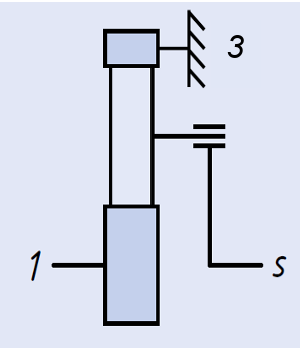
\includegraphics[width=0.23\linewidth,keepaspectratio]{graphics/v3_planetengetriebe_hohlrad_fest_n3_0.png}
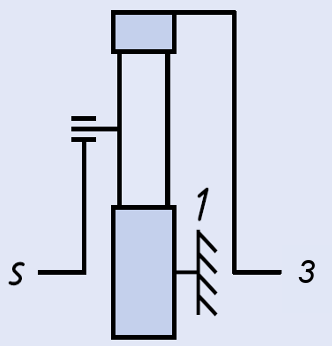
\includegraphics[width=0.25\linewidth,keepaspectratio]{graphics/v3_planetengetriebe_sonne_fest_n1_0.png}
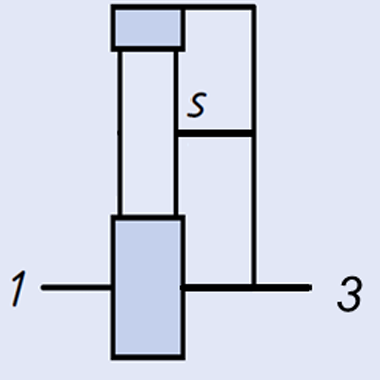
\includegraphics[width=0.24\linewidth,keepaspectratio]{graphics/v3_planetengetriebe_gleichlauf_n1_ns_n3.png}
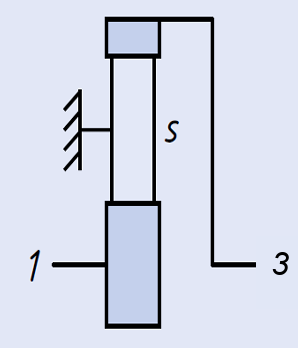
\includegraphics[width=0.23\linewidth,keepaspectratio]{graphics/v3_planetengetriebe_steg_fest_ns_0.png}
\end{figbox}
